\section{System Architecture and Methodology}
\label{sec:methodology}

\begin{figure}[htbp]
    \centering
    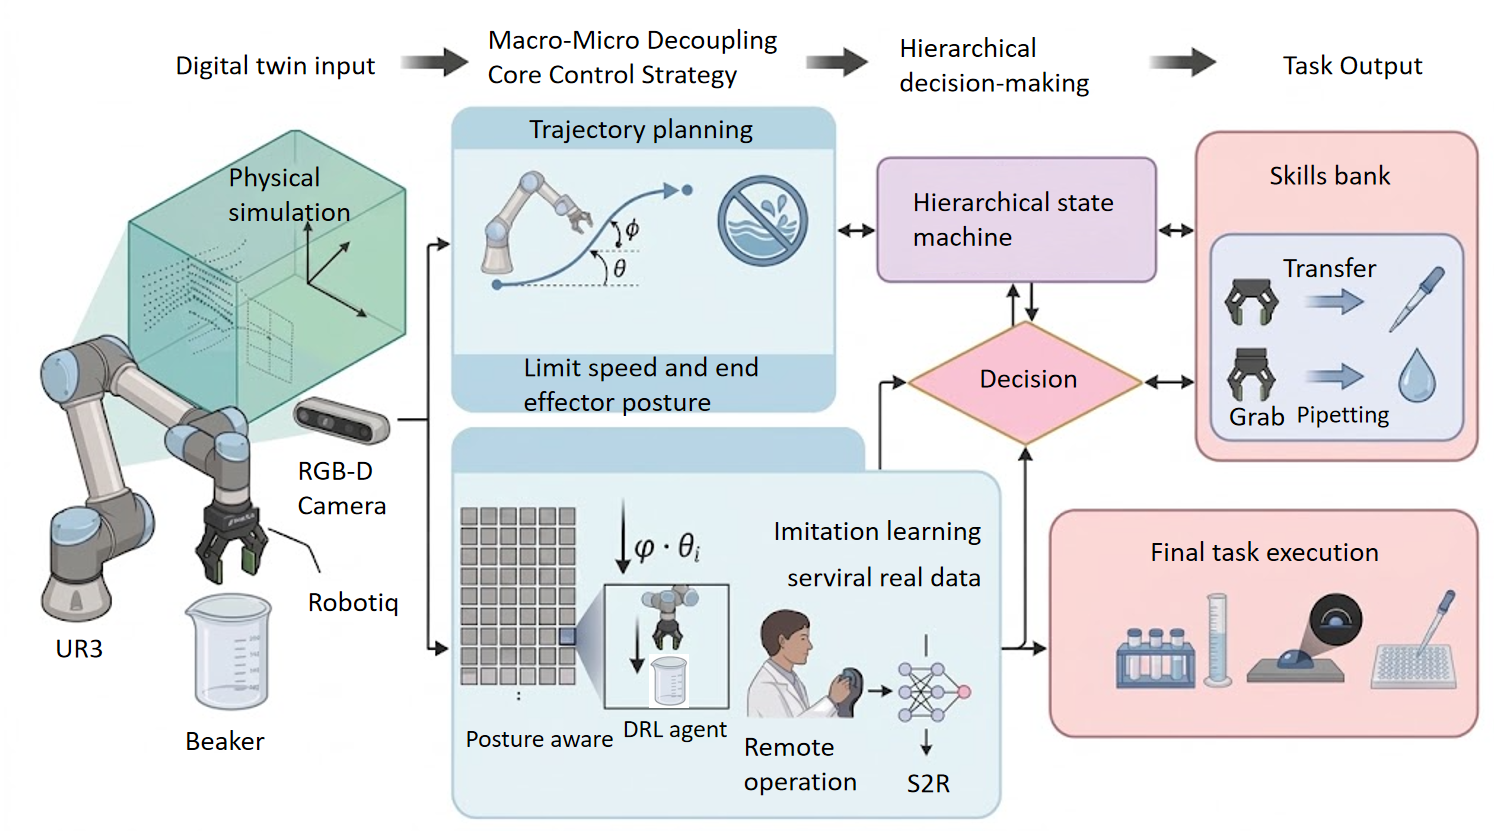
\includegraphics[width=\linewidth]{images/Framework.png}
    \caption{Multi-platform hybrid robotic end-to-end operation framework. The system employs a macro-micro decoupled strategy: macroscopic transit is controlled by a constraint-aware classical planner to ensure absolute spill-free safety, while microscopic contact-rich tasks are executed by neural network policies found within the rl file.}
    \label{fig:overall_framework}
\end{figure}

This section details the proposed multi-platform hybrid robotic framework tailored for automated bio-chemical assays, including solution preparation, contact angle detection, and serial dilution. To handle heterogeneous task requirements, macroscopic inter-station transit is executed via constraint-aware classical planning, while dexterous robotic arm manipulations are governed by a hybrid learning architecture combining massively parallel Deep Reinforcement Learning (DRL) and human-in-the-loop Imitation Learning (IL).

\subsection{Simulation Environment for Policy Training}
\label{subsec:simulation_training}

To enable risk-free training and pre-verification of contact-rich tasks, we construct a high-fidelity simulation environment using NVIDIA Isaac Sim. Powered by a GPU-accelerated tensor physics engine, the simulation environment accurately models rigid-body dynamics, joint torques, and frictional contacts. Signed Distance Field (SDF) collision meshes are assigned to gripper fingers and labware holders for penetration-free contact simulation. Crucially, the standalone Python API architecture enables GPU-based parallelization across thousands of simultaneous virtual environments, bypassing the sample inefficiency bottleneck of physical robotic learning.

\subsection{State Synchronization Between Simulation and Physical Environments}
\label{subsec:state_sync}

We define a state interface between the physical robot and the Isaac Sim environment. Joint encoders provide arm positions $\mathbf q_t$ and velocities $\dot{\mathbf q}_t$; the gripper reports opening and grasp confirmation. RGB-D observations provide each visible object's position $\mathbf p_{i,t}$, orientation $\mathbf R_{i,t}$, and detection confidence. Object velocity is estimated only when consecutive reliable observations are available. Each record retains its acquisition timestamp and source, so the simulator can distinguish a measured state from an estimated one.

Before updating the simulation, camera observations are transformed into the robot-base frame using calibrated extrinsics, and robot and object samples are aligned to a common timestamp. Joint positions are interpolated between encoder samples; object poses are updated from the latest valid visual observation. During brief occlusion after a force-confirmed grasp, the held object's pose is propagated from the end-effector pose and the measured grasp transform. The interface rejects stale or low-confidence object observations instead of presenting them as current measurements. These synchronized states support visualization and comparison of simulated and physical trajectories; they do not, by themselves, establish predictive accuracy or closed-loop control performance.

\subsection{Constraint-Aware Motion Planning for Macroscopic Navigation}
\label{subsec:macro_planning}

\begin{figure}[htbp]
    \centering
    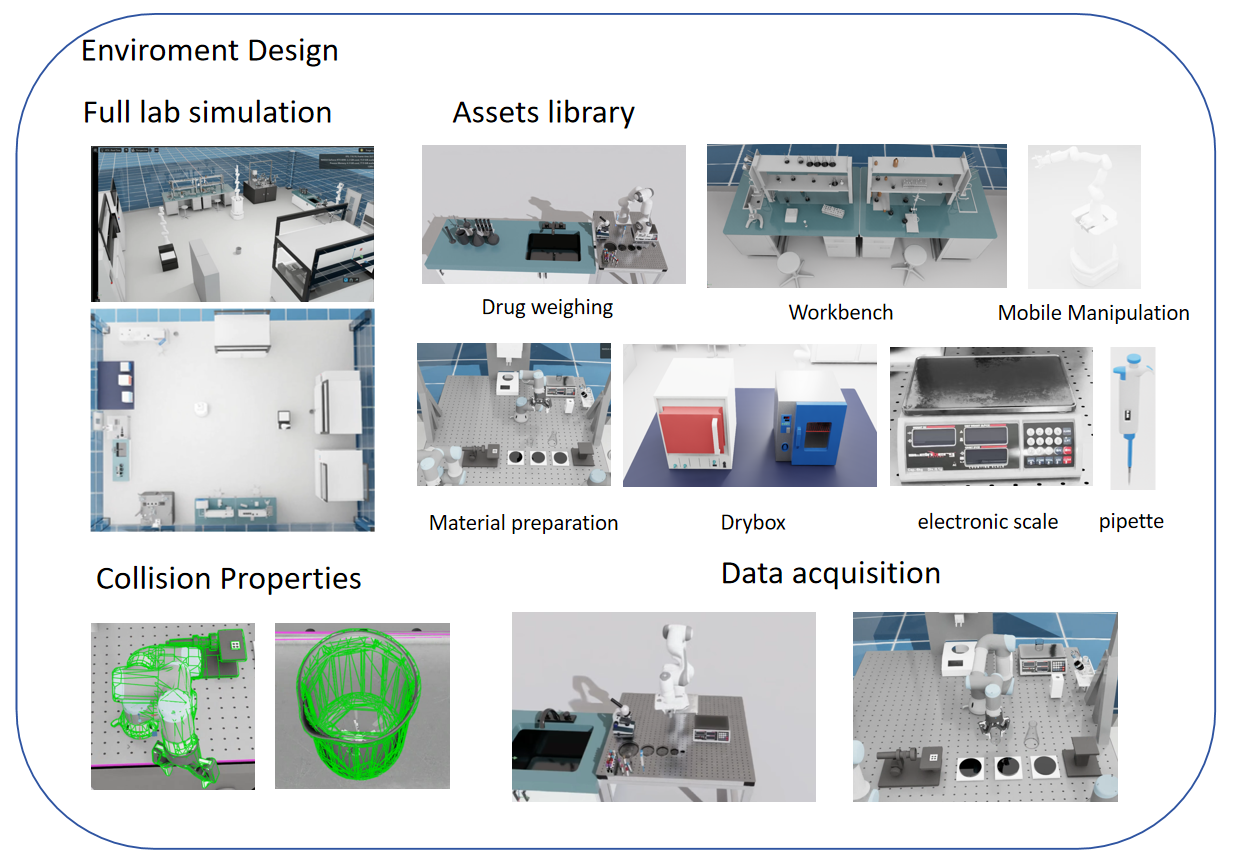
\includegraphics[width=0.9\linewidth]{images/environment_design.png}
    \caption{High-fidelity simulation environment built upon Isaac Sim. This simulation environment integrates a UR3 manipulator and a Robotiq 2F-85 parallel gripper, and employs Signed Distance Field (SDF) collision meshes to achieve accurate contact modeling .}
    \label{fig:sim_env}
\end{figure}

For macroscopic transit between workstations (e.g., carrying prepared reagent vials), we employ a constraint-aware classical motion planner. To prevent fluid sloshing during movement, strict task-space orientation constraints are imposed on the end-effector roll ($\phi$) and pitch ($\theta$):
\begin{equation}
    |\phi(t) - \phi_{\text{target}}| \leq \epsilon_{\phi}, \quad |\theta(t) - \theta_{\text{target}}| \leq \epsilon_{\theta}, \quad \forall t \in [0, T]
\end{equation}
Path smoothing is formulated as a minimum-jerk trajectory optimization problem:
\begin{equation}
    \min_{q(t)} \int_{0}^{T} \left\| \dddot{q}(t) \right\|^2 dt
\end{equation}
subject to velocity ($\dot{q}_{\max}$) and acceleration ($\ddot{q}_{\max}$) bounds, guaranteeing smooth, collision-free container transit.

\subsection{Massively Parallel DRL with Posture-Aware Reward Engineering}
\label{subsec:arm_rl}

For labware grasping and lifting, explicitly modeling micro-contact dynamics is computationally intractable. We implement a Deep Reinforcement Learning (DRL) pipeline formulated as a Markov Decision Process (MDP), defined by the tuple $\mathcal{M} = (\mathcal{S}, \mathcal{A}, \mathcal{P}, \mathcal{R}, \gamma)$:

\begin{itemize}
    \item \textbf{State Space} $\mathcal{S}$: At each time step $t$, the state observation $s_t \in \mathcal{S}$ is composed of:
    \begin{equation}
        s_t = [\mathbf{q}_t, \dot{\mathbf{q}}_t, \mathbf{p}_{ee}, \mathbf{R}_{ee}, \mathbf{p}_{obj}, \mathbf{R}_{obj}, g_t]
    \end{equation}
    where $\mathbf{q}_t \in \mathbb{R}^6$ denotes joint positions, $\dot{\mathbf{q}}_t \in \mathbb{R}^6$ denotes joint velocities, $\mathbf{p}_{ee} \in \mathbb{R}^3$ and $\mathbf{R}_{ee} \in SO(3)$ represent the end-effector pose, $\mathbf{p}_{obj} \in \mathbb{R}^3$ and $\mathbf{R}_{obj} \in SO(3)$ denote the object pose, and $g_t \in \{0, 1\}$ is the gripper state.

    \item \textbf{Action Space} $\mathcal{A}$: The continuous action $a_t \in \mathcal{A}$ consists of:
    \begin{equation}
        a_t = [\Delta\mathbf{q}_t, \Delta g_t] \in \mathbb{R}^7
    \end{equation}
    where $\Delta\mathbf{q}_t \in \mathbb{R}^6$ represents joint velocity commands and $\Delta g_t \in [-1, 1]$ controls gripper opening/closing.

    \item \textbf{Transition Dynamics} $\mathcal{P}$: The state transition probability $\mathcal{P}(s_{t+1}|s_t, a_t)$ is governed by the physics engine simulation.

    \item \textbf{Reward Function} $\mathcal{R}$: The reward signal $r_t = \mathcal{R}(s_t, a_t)$ is designed to guide the policy toward successful grasping (detailed in Section~\ref{subsec:reward_design}).

    \item \textbf{Discount Factor} $\gamma \in [0, 1)$: Balances immediate and future rewards.
\end{itemize}

\begin{figure}[htbp]
    \centering
    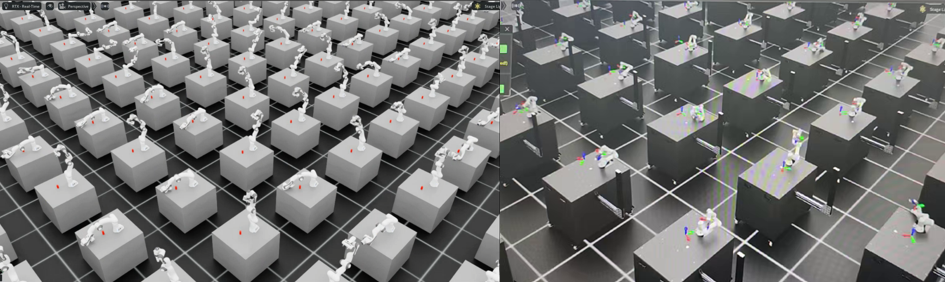
\includegraphics[width=0.9\linewidth]{images/Large scale parallel training.png}
    \caption{High-fidelity simulation environment built upon Isaac Sim. This simulation environment integrates a UR3 manipulator and a Robotiq 2F-85 parallel gripper, and employs Signed Distance Field (SDF) collision meshes to achieve accurate contact modeling .}
    \label{fig:sim_env_parallel}
\end{figure}

\subsubsection{Reward Function Design}
\label{subsec:reward_design}

To prevent liquid container tilting during grasping, we design a dense reward function with a \textit{posture-aware multiplier}. Let $\mathbf{z}_{\text{curr}}$ denote the normalized local z-axis vector of the object, and $\mathbf{z}_{\text{target}} = [0, 0, -1]^T$ denote the ideal downward vector. The posture multiplier $M_{\text{posture}}$ is defined as:
\begin{equation}
    M_{\text{posture}} = \text{clamp}(\mathbf{z}_{\text{curr}} \cdot \mathbf{z}_{\text{target}}, \, 0.0, \, 1.0)
\end{equation}

The complete reward function at each time step is composed of multiple components:
\begin{equation}
    R_t = \underbrace{R_{\text{distance}}}_{\text{approach}} + \underbrace{R_{\text{grasp}}}_{\text{grasping}} + \underbrace{R_{\text{lift}}}_{\text{lifting}} - \underbrace{R_{\text{collision}}}_{\text{penalty}}
\end{equation}

where each component is defined as:
\begin{align}
    R_{\text{distance}} &= -\alpha_1 \left\| \mathbf{p}_{ee} - \mathbf{p}_{obj} \right\|_2 \cdot M_{\text{posture}} \\
    R_{\text{grasp}} &= \alpha_2 \cdot \mathbb{I}[\text{grasped}] \cdot M_{\text{posture}} \\
    R_{\text{lift}} &= \alpha_3 \cdot (z_{obj} - z_{obj,0}) \cdot M_{\text{posture}} \\
    R_{\text{collision}} &= \alpha_4 \cdot \mathbb{I}[\text{collision}]
\end{align}

where $\alpha_1, \alpha_2, \alpha_3, \alpha_4$ are weighting coefficients, $\mathbb{I}[\cdot]$ is the indicator function, and $z_{obj,0}$ is the initial object height. If the container tilts beyond $90^\circ$, $M_{\text{posture}}$ collapses to zero, heavily penalizing improper orientations and forcing the policy to master upright grasping.

\subsubsection{PPO Optimization}
\label{subsec:ppo}

Training is accelerated using Proximal Policy Optimization (PPO) distributed across 4,096 parallel virtual environments in Isaac Sim. The PPO clipped surrogate objective is defined as:
\begin{equation}
    L^{CLIP}(\theta) = \hat{\mathbb{E}}_t \left[ \min \left( r_t(\theta) \hat{A}_t, \, \text{clip}(r_t(\theta), 1-\epsilon, 1+\epsilon) \hat{A}_t \right) \right]
\end{equation}

where $r_t(\theta) = \frac{\pi_\theta(a_t|s_t)}{\pi_{\theta_{old}}(a_t|s_t)}$ is the probability ratio, $\hat{A}_t$ is the estimated advantage function computed using Generalized Advantage Estimation (GAE):
\begin{equation}
    \hat{A}_t = \sum_{l=0}^{T-t} (\gamma \lambda)^l \delta_{t+l}, \quad \delta_t = r_t + \gamma V(s_{t+1}) - V(s_t)
\end{equation}

The total loss function combines the clipped surrogate with value function and entropy bonuses:
\begin{equation}
    L(\theta) = L^{CLIP}(\theta) - c_1 L^{VF}(\theta) + c_2 H[\pi_\theta](s_t)
\end{equation}

where $L^{VF} = (V_\theta(s_t) - V_t^{\text{target}})^2$ is the value function loss, $H[\pi_\theta]$ is the entropy bonus encouraging exploration, and $c_1, c_2$ are coefficients.

The training hyperparameters are summarized in Table~\ref{tab:hyperparameters}.

\begin{table}[!t]
\renewcommand{\arraystretch}{1.3}
\caption{Training Hyperparameters for PPO}
\label{tab:hyperparameters}
\centering
\begin{tabular}{lc}
\hline\hline
\textbf{Hyperparameter} & \textbf{Value} \\ \hline
Learning Rate & $3 \times 10^{-4}$ \\
Discount Factor $\gamma$ & 0.99 \\
GAE Parameter $\lambda$ & 0.95 \\
Clip Parameter $\epsilon$ & 0.2 \\
Entropy Coefficient $c_2$ & 0.01 \\
Value Loss Coefficient $c_1$ & 0.5 \\
Batch Size & 4096 \\
Mini-Batch Size & 512 \\
Epochs per Update & 10 \\
Max Gradient Norm & 0.5 \\
Number of Environments & 4096 \\
Training Iterations & 5000 \\ \hline\hline
\end{tabular}
\end{table}

\subsubsection{Domain Randomization}
\label{subsec:domain_randomization}

To bridge the sim-to-real gap, we apply extensive domain randomization during training. The randomized parameters $\theta_{DR}$ are sampled from uniform distributions:
\begin{equation}
    \theta_{DR} \sim \mathcal{U}(\theta_{\text{base}} - \Delta\theta, \, \theta_{\text{base}} + \Delta\theta)
\end{equation}

The specific randomization ranges are detailed in Table~\ref{tab:domain_randomization}.

\begin{table}[!t]
\renewcommand{\arraystretch}{1.3}
\caption{Domain Randomization Parameters}
\label{tab:domain_randomization}
\centering
\begin{tabular}{lcc}
\hline\hline
\textbf{Parameter} & \textbf{Base Value} & \textbf{Range} \\ \hline
Table Friction & 0.5 & $[0.3, 0.8]$ \\
Object Mass (g) & 100 & $[80, 130]$ \\
Gripper Friction & 0.8 & $[0.5, 1.2]$ \\
Light Intensity & 1.0 & $[0.6, 1.4]$ \\
Camera Position (cm) & -- & $\pm 5$ \\
Object Position (cm) & -- & $\pm 3$ \\ \hline\hline
\end{tabular}
\end{table}

\subsection{Imitation Learning and Few-Shot Sim-to-Real Fine-Tuning}
\label{subsec:arm_il_adaptation}

For precision-critical micro-manipulations such as micro-pipetting and droplet dispensing, we introduce a teleoperation-guided Imitation Learning (IL) pipeline. Expert demonstrations $\mathcal{D}_{\text{sim}} = \{(s_t, a_t)\}_{i=1}^N$ are collected within the simulation environment using a 6-DoF SpaceMouse interface. A visuomotor policy $\pi_\theta(a_t | s_t)$ is pre-trained via Behavioral Cloning (BC):
\begin{equation}
    \mathcal{L}_{\text{BC}}(\theta) = \mathbb{E}_{(s_t, a_t) \sim \mathcal{D}_{\text{sim}}} \left[ \left\| \pi_\theta(s_t) - a_t \right\|_2^2 \right]
\end{equation}
During simulation training, Domain Randomization (DR) is applied to lighting, visual textures, object mass, and friction coefficients $\mu \sim \mathcal{U}(\mu_{\min}, \mu_{\max})$.

To bridge real-world reality gaps caused by liquid surface tension, refractive optics, and gripper compliance, we implement a regularized few-shot real-world fine-tuning mechanism using $M$ physical demonstrations ($M \ll N$). The policy parameters adapt to $\theta_{\text{real}}$ by minimizing:
\begin{equation}
    \theta_{\text{real}} = \arg\min_{\theta} \left( \mathbb{E}_{(s_t, a_t) \sim \mathcal{D}_{\text{real}}} \left[ \left\| \pi_\theta(s_t) - a_t \right\|_2^2 \right] + \lambda \left\| \theta - \theta_{\text{sim}} \right\|_2^2 \right)
\end{equation}
where $\lambda$ is a regularization hyperparameter that prevents catastrophic forgetting of features learned in simulation, achieving robust physical deployment.

\subsection{Failure-Aware Hierarchical State Machine and Skill Library}
\label{subsec:hierarchical_skill}

To coordinate a multi-stage bio-assay, we use a rule-based hierarchical state machine (HSM) above a modular \textit{Skill Library}. The HSM is not a learned high-level reinforcement-learning policy. It separates task sequencing from low-level control and makes transition and recovery conditions explicit.

The library $\mathcal{L}_{\text{skills}} = \{\pi_{\text{grasp}}, \pi_{\text{transit}}, \pi_{\text{pour}}, \dots\}$ contains independently implemented manipulation policies and classical planning routines. Each skill declares preconditions, a completion guard, a timeout, and a failure code. Modularity permits one skill to be changed without retraining every other skill, but prevention of negative transfer is not claimed without a monolithic-policy comparison.

\begin{figure}[htbp]
    \centering
    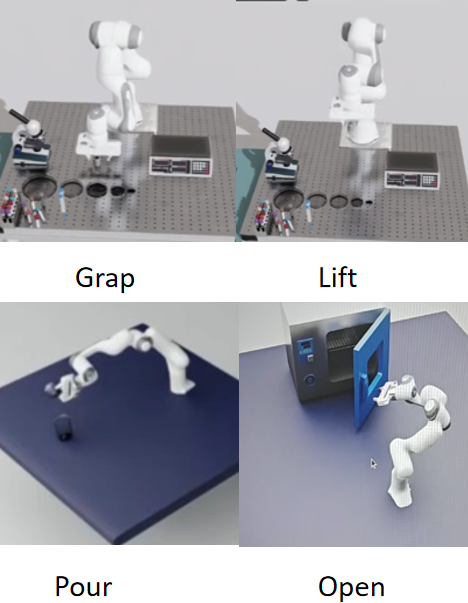
\includegraphics[width=0.5\linewidth]{images/skill_lab.png}
    \caption{Autonomous characterization workflow governed by a Hierarchical State Machine (HSM) and a modular skill library. By invoking reusable low-level skill primitives, the system successfully executes comprehensive, multi-stage experimental cycles without human intervention.}
    \label{fig:skill_library}
\end{figure}

The HSM has states such as \texttt{approach}, \texttt{grasp}, \texttt{verify}, \texttt{transit}, \texttt{handover}, and \texttt{recover}. At each transition, predefined guards evaluate observable signals such as \texttt{is\_bottle\_grasped}, \texttt{is\_at\_target}, docking confirmation, and sensor freshness. The transition function $s_{t+1}=\delta(s_t,g(o_t))$ is deterministic given the current HSM state and guard outcomes; no transition probabilities or learned confidence scores are assumed.

If grasp verification fails, the HSM stops transit and returns to \texttt{grasp} after a safe repositioning action. A retry counter and timeout bound repeated attempts; exhaustion moves the system to a safe-stop state for operator review. This is a specified recovery mechanism, not evidence of an improved recovery rate. Its contribution should be evaluated against a fixed sequential state machine without recovery, using stage-level and full-workflow success, recovery attempts, intervention count, and completion time.

Containers are transferred between the mobile platform and workstation manipulators at designated task stages. The task sequence records transfer completion before proceeding.
